\section{Introduction}

Cancer represents the most significant global health challenge \cite{siegel2023cancer}. Furthermore, according to the Cancer Research Institute of the United Kingdom, more than 18 million new cases and 10 million deaths were recorded in 2020 \cite{cancerUK2023}. Furthermore, it is predicted that there will be 28 million new cases annually by around 2040 if the incidence remains stable, and population growth and aging continue according to recent trends \cite{cancerUK2023_2}. This represents a 54.9\% increase from 2020, with the increase expected to be higher in men (60.6\%) than in women (48.8\%). In this context, it is well known that traditional methods based on surgery, radiotherapy, and chemotherapy have low efficacy and adverse side effects \cite{peng2019neoantigen}. Thus, the development of cancer immunotherapy has emerged, aiming to stimulate the immune system of the patient \cite{borden2022cancer}. There are treatments like personalized vaccines, adoptive T-cell therapies, and immune checkpoint inhibitors. Among these, neoantigen-based vaccines have shown great potential by enhancing T-cell responses and are considered the most likely to succeed \cite{borden2022cancer}. Additionally, neoantigens are used in immune checkpoint blockade therapy. Neoantigens are considered predictive biomarkers and targets for synergistic treatment in cancer immunotherapy \cite{fang2022neoantigens}.


Despite various efforts in the development of neoantigen detection methods, less than 5\% of detected neoantigens activate the immune system, as reported by several studies \cite{de2020neoantigen, mill2022neoms, bulik2019deep, bassani2015mass, yadav2014predicting}. The reasons are related to: the no integration of multiple data sources like DNA-seq, RNA-seq, and Mass Spectrometry (MS) \cite{kim2018neopepsee}. Use of low-performance tools for peptide-MHC binding prediction like MHCFlurry \cite{o2020mhcflurry} and NetMHCpan4.1 \cite{reynisson2020netmhcpan}. Neglecting the prediction of pMHC-TCR binding \cite{rubinsteyn2018computational}. Overlooking information from alternative splicing events, structural DNA variants, and gene fusion mutations, this information is closely related to various types of cancer \cite{wood2020neoepiscope}.


\begin{figure}[h]
	
	\begin{subfigure}[b]{0.4\textwidth}
		\centering
		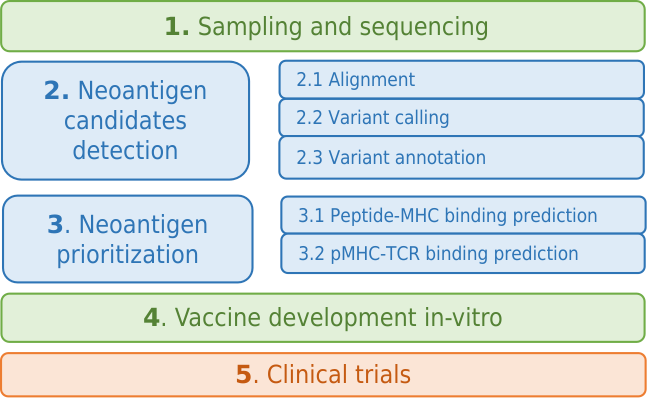
\includegraphics[width=\textwidth]{../img/proposal/vaccine_pipeline}
		\caption{Vaccine process development}
		\label{fig:pipeline_a}
	\end{subfigure}
	\hfill
	\begin{subfigure}[b]{0.55\textwidth}
		\centering
		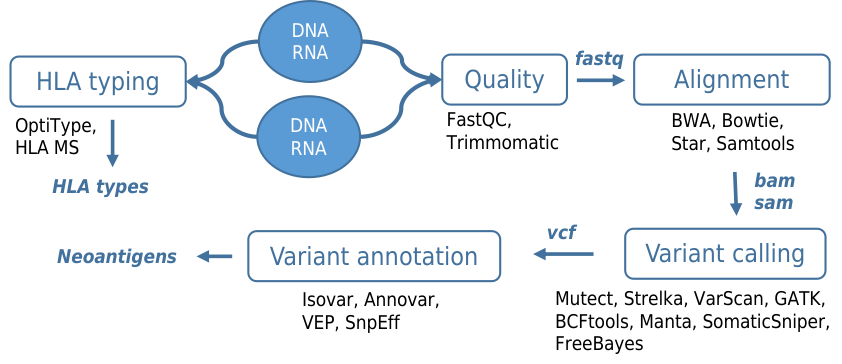
\includegraphics[width=\textwidth]{../img/proposal/neoantigen_detection}
		\caption{Neoantigen detection process}
		\label{fig:pipeline_b}
	\end{subfigure}
	\hfill
	
	\caption{(a) The process to detect neoantigens and develop personalized vaccines. It starts with DNA-seq or RNA-seq; then, neoantigen detection is performed, followed by neoantigen prioritization; subsequently, a personalized vaccine is developed \textit{in vitro}; and clinical trials are applied. (b) Process for the Detection of Neoantigen Candidates Initially, DNA/RNA sequencing is conducted on both tumor and normal cells. Subsequently, quality assessment tools are employed, followed by the utilization of alignment tools. The process then proceeds to variant calling to identify variants. Finally, variant annotation tools are applied to generate a list of potential neoantigen candidates. Moreover, MHC typing tools are employed to determine the HLA or MHC types.}
	\label{fig:pipeline}
\end{figure}

\textbf{Neoantigen detection} relies on an initial identification of candidates, which is followed by their subsequent prioritization (stages two and three of Fig. \ref{fig:pipeline_a}). In this project, the vaccine development and clinical trials are out of the scope; however, they will be included in future works. Detection of neoantigen candidates involves a multi-step process (see Fig. \ref{fig:pipeline_b}). DNA/RNA sequencing is initially conducted on both tumor and normal cells. Subsequently, quality assessment tools are employed, followed by the utilization of alignment tools. The process then proceeds to variant calling to identify genetic variants. Finally, variant annotation tools are applied to generate a list of potential neoantigen candidates. In addition to the aforementioned steps, quantitative proteomic tools are utilized for mass spectrometry (MS) data analysis. Moreover, MHC typing tools are employed to determine the Human Leukocyte Antigen (HLA) or Major Histocompatibility Complex (MHC) types.

\textbf{Neoantigen prioritization} is the third stage in cancer vaccines development (Fig. \ref{fig:pipeline_a}). This stage takes candidates' neoantigens and then predicts their affinity to the Major Histocompatibility Complex (MHC); this problem is known as the pMHC binding prediction problem. Then,  this pMHC complex is used to predict the interaction with the T-cell Receptor (TCR). Both problems take two protein sequences as input, and the goal is to predict their affinity (regression) or binding (classification). In summary, the proteins can be represented as $p = \{ A, ... , Q \}$ and  $q = \{ A, N, K, L, ... ,Q \}$. Then, we need to know the probability of affinity between $p$ and $q$. 

Thus, in this project, a method for neoantigen prioritization using Transformer and Transfer Learning is proposed. This method relies on the prediction of pMHC bindings. Moreover, the proposal fine-tuned six pre-trained BERT models, adding a block of BiLSTM at the end. Moreover, HLAB dataset \cite{zhang2022hlab} was used for training and testing. Additionally, a layer freezing methodology along with Gradient Accumulation Steps were applied. According to our results, ArgosMHC got promising results outperforming state-of-arts tools like NetMHCpan4.1 \cite{reynisson2020netmhcpan}, MHCFlurry2.0 \cite{o2020mhcflurry}, Anthem \cite{mei2021anthem}, Acme \cite{hu2019acme}, and MixMHCpred2.2 \cite{gfeller2023improved}.
